\chapter{Process Automation}

\section{Process Design}

We selected main features of this part of the law and designed BPMN model.

\begin{landscape}

    \begin{figure}[h]\centering
        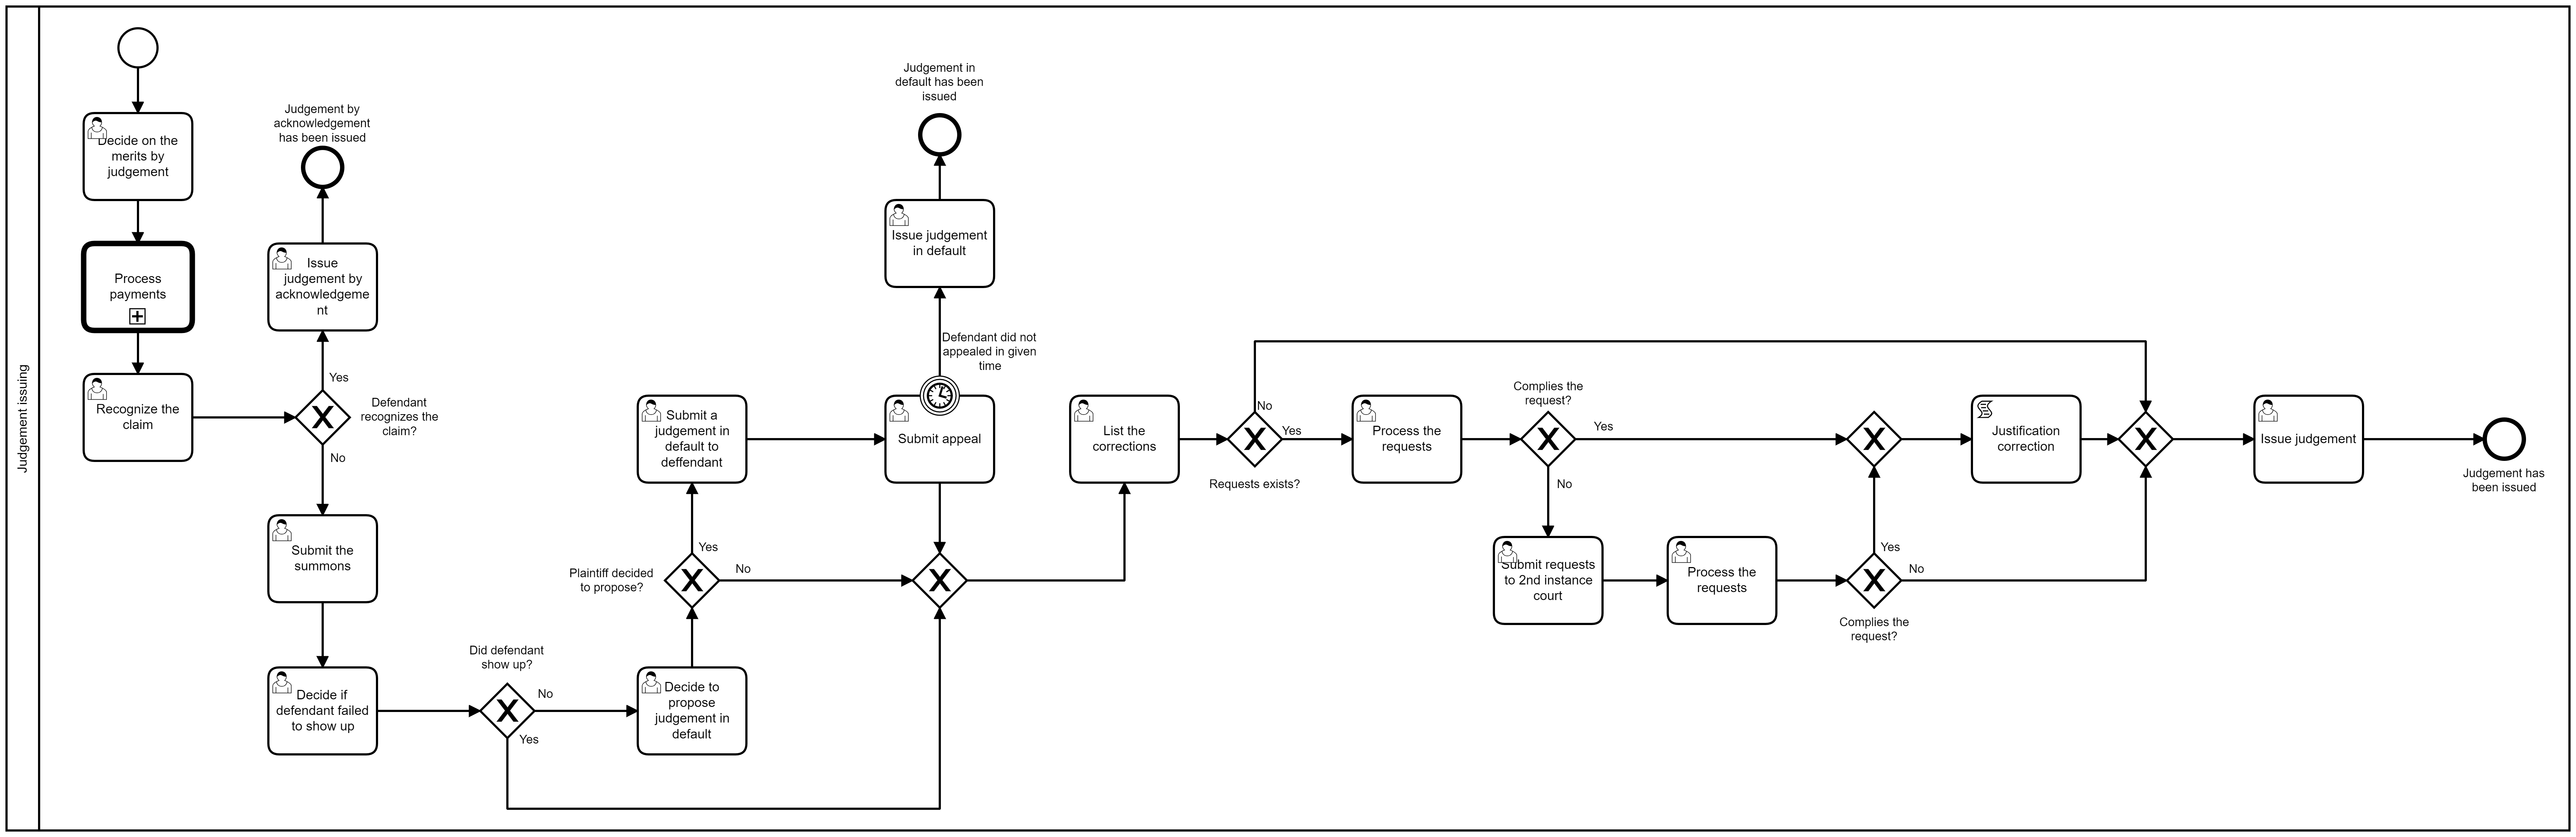
\includegraphics[width=22cm]{pic/bpmn}
        \caption{BPMN main diagram}
        \label{fig:bpmnModel}
    \end{figure}
    
    \begin{figure}[h]\centering
        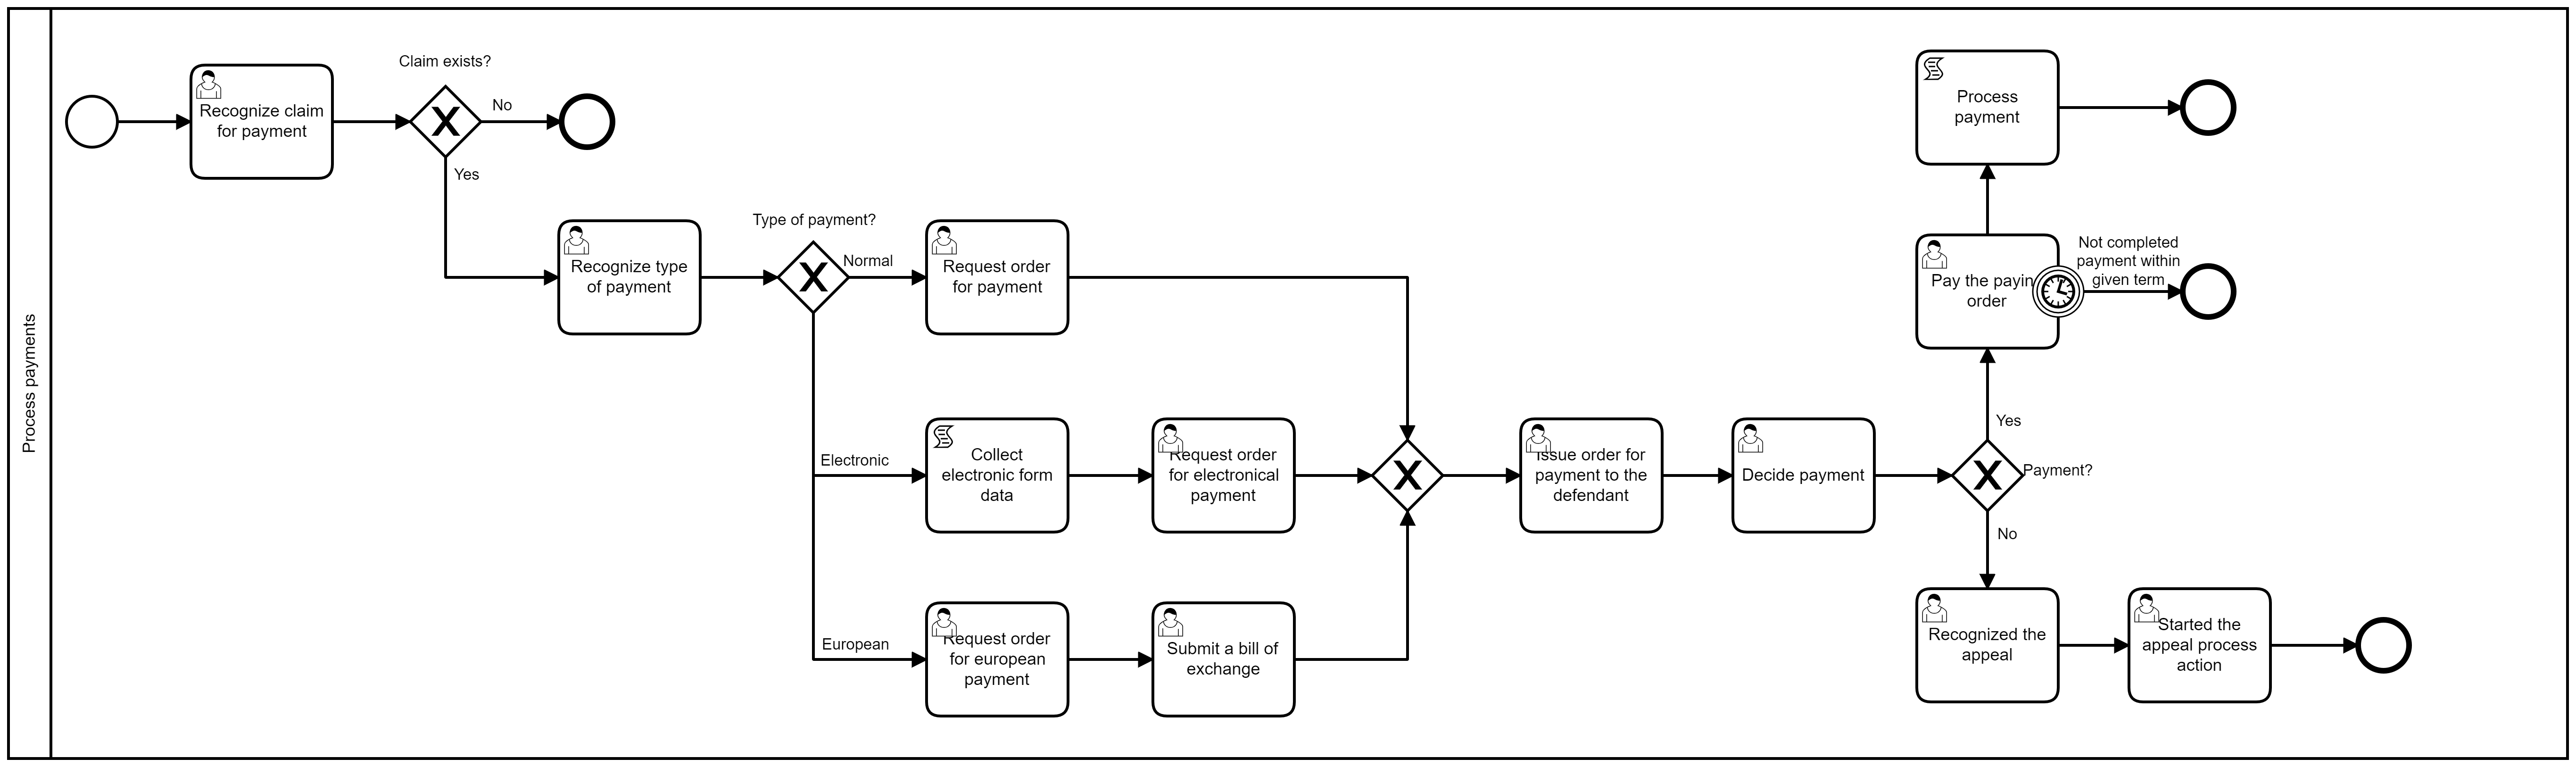
\includegraphics[width=22cm]{pic/bpmn_payments}
        \caption{BPMN payments diagram}
        \label{fig:bpmnPaymentsModel}
    \end{figure}
    
    \end{landscape}
    
    \section{Process Execution}
    
    We also tested the BPMN model in Camunda platform. Figures below shows some of the steps of the process.
    
    \begin{landscape}
        
        \begin{figure}[h]\centering
            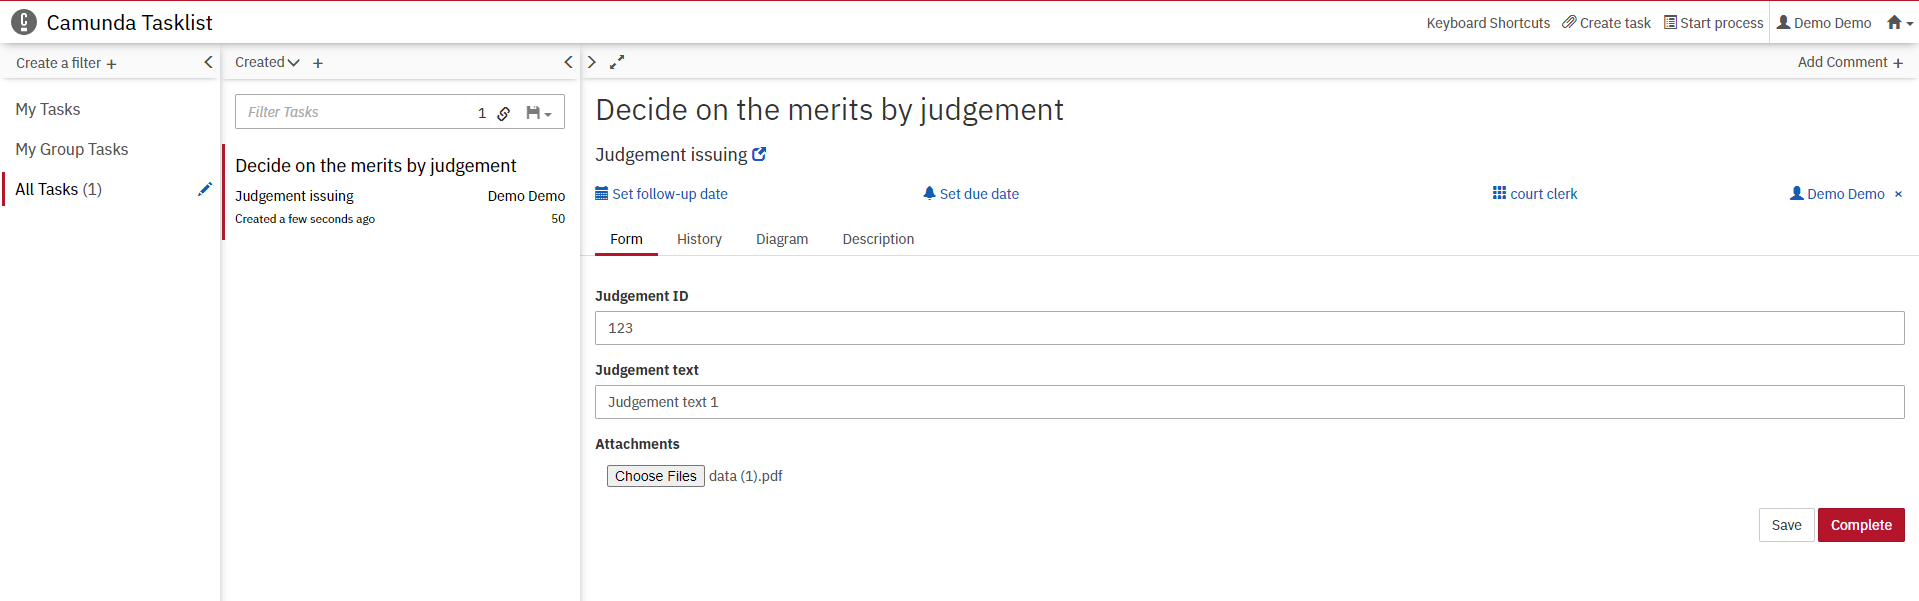
\includegraphics[width=22cm]{pic/camunda1}
            \caption{BPMN form: decide on the merits by judgement}
            \label{fig:camunda1}
        \end{figure}
    
        \begin{figure}[h]\centering
            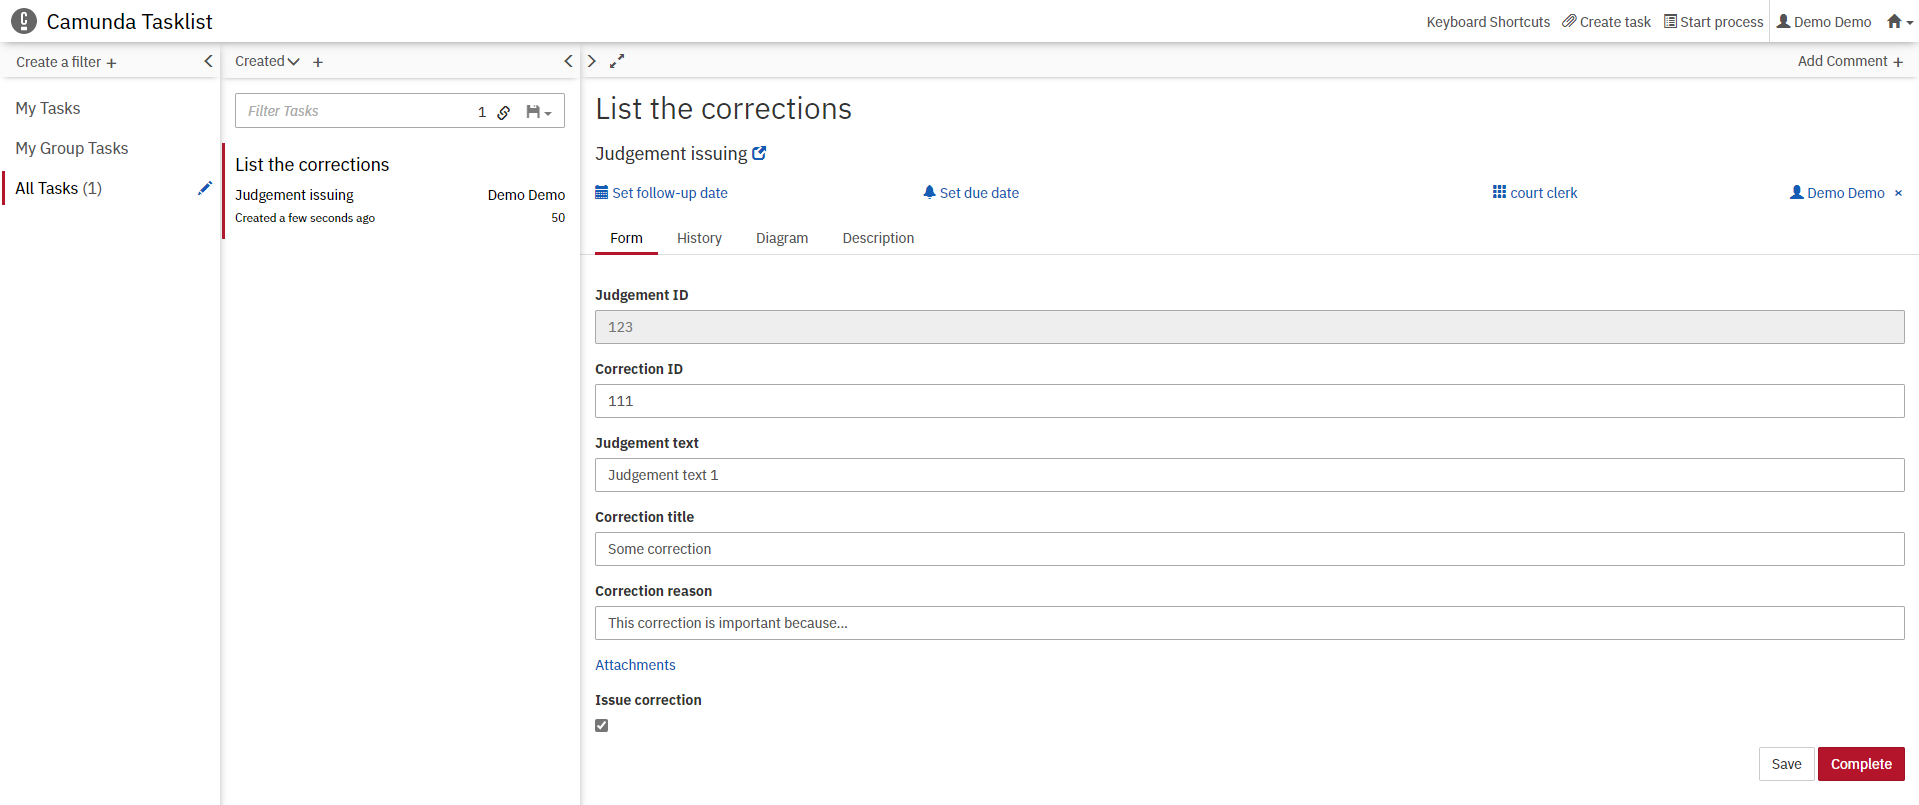
\includegraphics[width=22cm]{pic/camunda2}
            \caption{BPMN form: list the corrections}
            \label{fig:camunda2}
        \end{figure}
    
        \begin{figure}[h]\centering
            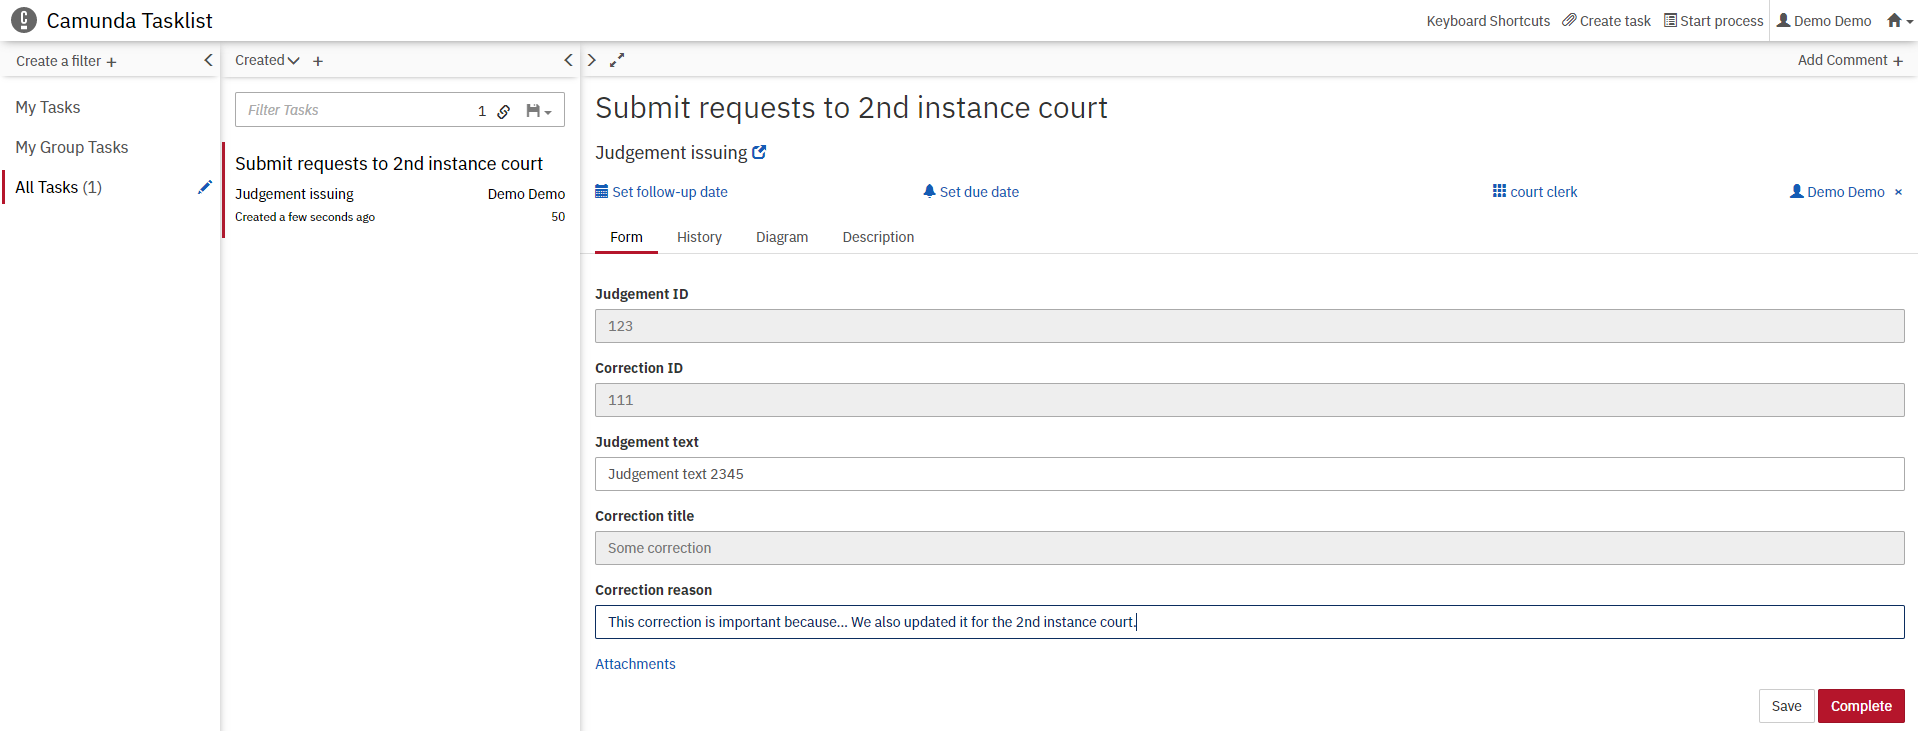
\includegraphics[width=22cm]{pic/camunda3}
            \caption{BPMN form: submit requests to 2nd instance court}
            \label{fig:camunda3}
        \end{figure}
    
        \begin{figure}[h]\centering
            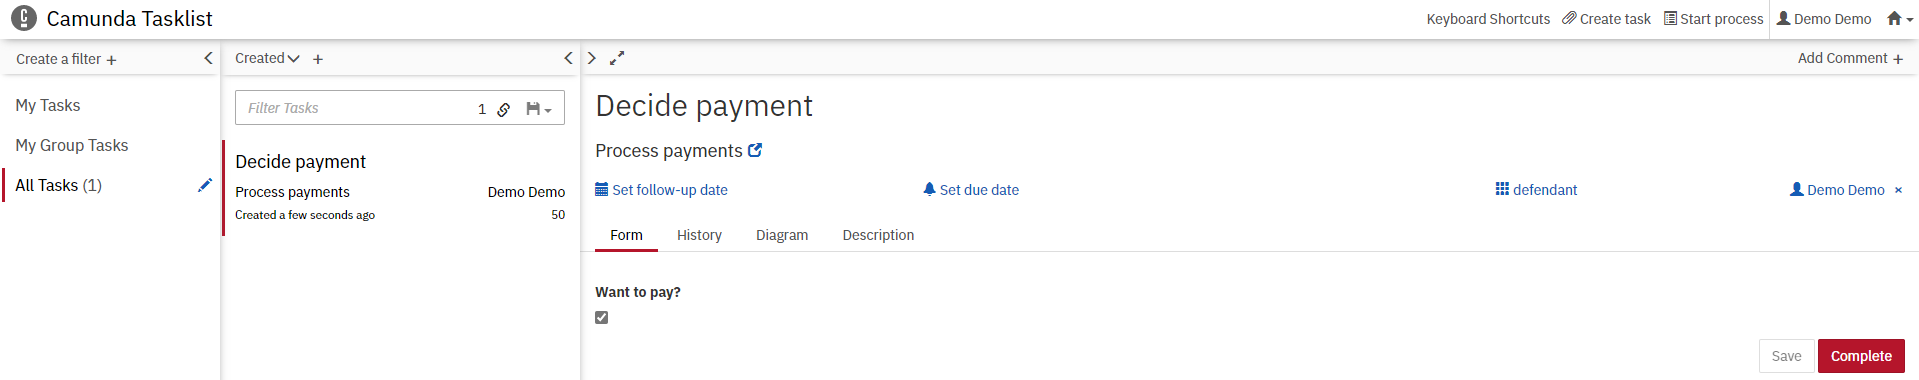
\includegraphics[width=22cm]{pic/camunda4}
            \caption{BPMN form: Decide to pay}
            \label{fig:camunda4}
        \end{figure}
    
    \end{landscape}

\section{Results Presentation}\label{sec:presentation}

An url to our presentation video: \url{https://www.youtube.com/watch?v=qfprck_Djro}
